\section{Improvements II: Computation}
\label{sec:impcompute}

The original kernel code is correct but very slow. It is so slow that it ruled out the
experiments needed to answer the project's own research question: repeated runs, tuning,
ablations, and realistic training-set sizes at 16 qubits. This section describes three changes
that keep the exact same kernel values while removing the bottleneck.

\subsection{Simulate each sample once (statevector caching)}
\paragraph{Problem.} \code{\_kernel\_statevector(a, b)} simulated $U(\bm a)\ket0$ and
$U(\bm b)\ket0$ from scratch for every pair. For $N$ training and $M$ test samples the original
code performed
\begin{equation}
\underbrace{2\cdot\tfrac{N(N+1)}{2}}_{K_\text{train}}+\underbrace{2\cdot 2MN}_{K_\text{test}\ \text{in predict and predict\_proba}}
\end{equation}
circuit simulations: about 5.1 million for $N=1600$, $M=400$. Yet $\ket{\phi(\bm x)}$ depends
only on $\bm x$.

\paragraph{Change.} \code{QuantumKernel.states(X)} returns the matrix $\Phi_X\in\mathbb{C}^{N\times2^n}$
whose rows are the feature states. The whole kernel matrix is then one matrix product:
\begin{equation}
K(X,Y)=\big|\,\overline{\Phi_X}\,\Phi_Y^{\top}\big|^{\circ2}\qquad(\text{element-wise squared modulus}).
\label{eq:gram}
\end{equation}
This needs $N+M$ state preparations and one complex GEMM (\code{cgemm} in OpenBLAS, multithreaded),
computed in row blocks of 512 to bound memory. The most recent two state matrices are memoised.
When the test kernel is built, the training states are reused rather than re-simulated, and
\code{QSVM.predict}, \code{predict\_proba} and \code{decision\_function} share one cached test
kernel. With the Cirq backend this alone cuts the 16-qubit cost from about 44 hours to about
a minute (Table~\ref{tab:speed}).

\subsection{An exact fast engine for the ZZ feature map}
Cirq is a general-purpose simulator. It applies each of the $\approx\!4n$ gates per repetition as
a separate tensor contraction, with Python overhead per gate and per circuit. The ZZ map has
special structure that a dedicated engine can use.

\begin{proposition}
Let $s_i(z)=1-2z_i$ and
\begin{equation}
\Phi_{\bm x}(z)=\sum_{i=1}^n x_i\,s_i(z)+\sum_{(i,j)\in E}(\pi-x_i)(\pi-x_j)\,s_i(z)s_j(z).
\label{eq:phase}
\end{equation}
Then one repetition of the ZZ map is $U=D_{\bm x}H^{\otimes n}$ with $D_{\bm x}\ket z=e^{-i\Phi_{\bm x}(z)}\ket z$,
and the feature state after $r$ repetitions is
\begin{equation}
\ket{\phi_r(\bm x)}=D_{\bm x}H^{\otimes n}\cdots D_{\bm x}H^{\otimes n}\ket{0^n},\qquad
\ket{\phi_1(\bm x)}=2^{-n/2}\sum_z e^{-i\Phi_{\bm x}(z)}\ket z .
\end{equation}
\end{proposition}
\begin{proof}
$R_z(2x_i)$ acts on $\ket z$ as $e^{-ix_is_i(z)}$. By Eq.~\eqref{eq:zzgate}, the gate block for
pair $(i,j)$ acts as $e^{-i(\pi-x_i)(\pi-x_j)s_i(z)s_j(z)}$. All these operators are diagonal, so
they commute and their phases add, giving $D_{\bm x}$. Finally,
$H^{\otimes n}\ket{0^n}=2^{-n/2}\sum_z\ket z$.
\end{proof}

\paragraph{Implementation} (\code{FastZZStatevector} in \code{qsvm.py}).
\begin{enumerate}
\item \textbf{Phase table.} Precompute the sign matrix $S\in\{\pm1\}^{2^n\times n}$, with qubit 0
      as the most significant bit to match Cirq's ordering, and the pair-product matrix
      $S_P\in\{\pm1\}^{2^n\times|E|}$. For a batch of inputs $X$ (rows $\bm x$), all phases are
      two real matrix products:
      $\Phi = X S^\top + W S_P^\top$, where $W_{b,(i,j)}=(\pi-x_{b,i})(\pi-x_{b,j})$.
\item \textbf{First repetition} is free: $\psi=2^{-n/2}e^{-i\Phi}$, element-wise.
\item \textbf{Hadamard layers.} $H^{\otimes n}=H^{\otimes n_1}\otimes H^{\otimes n_2}$ with
      $n_1=\lfloor n/2\rfloor$. Reshaping $\psi$ into a $2^{n_1}\times2^{n_2}$ matrix $M$ (row-major)
      gives $(A\otimes B)\,\mathrm{vec}(M)=\mathrm{vec}(AMB^\top)$. Each layer is therefore two
      small batched matrix multiplications with $256\times256$ matrices at $n=16$, instead of a
      $65536\times65536$ operator or 16 strided butterfly passes.
\item Multiply by $D_{\bm x}$ again and repeat.
\end{enumerate}
The cost per sample is $O(2^n(n+|E|))$ for the phases and $O(2^n(2^{n_1}+2^{n_2}))$ per Hadamard
layer. Everything is vectorised over batches of 128 samples. States are stored as
\code{complex64}, the same precision Cirq uses by default.

\begin{algorithm}[H]
\caption{Training kernel with the fast engine}
\begin{algorithmic}
\STATE \textbf{input:} angles $A\in[0,\pi]^{N\times n}$, bandwidth $\alpha$, reps $r$, pairs $E$
\STATE $X\leftarrow\alpha A$
\FOR{each batch $B$ of 128 rows of $X$}
  \STATE $\Phi\leftarrow XS^\top+W(X)S_P^\top$;\quad $D\leftarrow e^{-i\Phi}$
  \STATE $\psi\leftarrow 2^{-n/2}D$
  \FOR{$k=2$ \TO $r$}
     \STATE $\psi\leftarrow \mathrm{vec}\big(H^{\otimes n_1}\,\mathrm{mat}(\psi)\,(H^{\otimes n_2})^{\top}\big)\odot D$
  \ENDFOR
  \STATE store $\psi$ as rows of $\Phi_X$
\ENDFOR
\STATE $K\leftarrow|\overline{\Phi_X}\Phi_X^\top|^{\circ 2}$;\quad symmetrise;\quad set $\operatorname{diag}(K)=1$
\end{algorithmic}
\end{algorithm}

\subsection{Other kernels on the same engine}
\paragraph{Separable $R_x$ kernel.} With the fast backend, Eq.~\eqref{eq:rxkernel} is evaluated
in closed form with broadcasting, in row blocks of 256. With the Cirq backend the product state
is simulated, which serves as a cross-check.

\paragraph{Finite shots.} Running $U^\dagger(\bm a)U(\bm b)$ for $s$ shots and counting the
all-zero outcomes gives a count distributed exactly as $\text{Binomial}(s, K(\bm a,\bm b))$: each
shot is an independent Bernoulli trial with success probability $|\bra{0^n}U^\dagger(\bm a)U(\bm b)\ket{0^n}|^2=K(\bm a,\bm b)$.
The fast backend therefore computes the exact kernel and draws
\begin{equation}
\hat K_{ij}=\frac1s\,\text{Binomial}\big(s,K_{ij}\big),
\end{equation}
independently for each upper-triangular entry, then mirrors it. This has \emph{the same
distribution} as the original sampling method at a tiny fraction of the cost. The real circuit
path is still available with \code{--backend cirq --sampling}. The estimator is unbiased
(verified in \code{test\_shot\_noise\_is\_unbiased}). The resulting matrix need not be PSD;
libsvm tolerates mildly indefinite kernels.

\subsection{Verification}
\label{sec:verify}
Speed is only useful if the numbers are unchanged. \code{tests/test\_core.py} checks:
\begin{itemize}
\item fast statevectors equal Cirq's (\code{atol} $10^{-5}$) for linear, circular and full
      entanglement, 2 and 3 repetitions, $\alpha=1$ and $\alpha=0.3$, and for the $R_x$ map.
      Observed maximum deviation: $2.4\times10^{-7}$, i.e.\ \code{float32} rounding;
\item the new kernel value equals the value from the \emph{original, unmodified}
      \code{legacy/qsvm.py} (\code{QuantumKernel(6,2).compute\_kernel\_value}) to 5 decimals;
\item Gram matrices are symmetric with unit diagonal, and their smallest eigenvalue is
      $>-10^{-5}$ (PSD up to rounding).
\end{itemize}
\code{main.py --backend cirq} and \code{--backend fast} produce identical predictions
(TESTING.md \S6).

\subsection{Speed}
Table~\ref{tab:speed} and Figure~\ref{fig:speed} compare the cost of the training ($1600^2$) plus
test ($400\times1600$) kernels. ``Original'' is extrapolated from the measured per-entry time of
\code{legacy/qsvm.py} times the number of entries it evaluates. ``Cirq cached'' is the measured
per-state Cirq time times 2000 states, plus the measured Gram-product time. ``Fast'' is measured
end to end.

\begin{table}[H]
\centering\small
\caption{Kernel computation cost, $N_\text{train}=1600$, $N_\text{test}=400$, 2 repetitions, linear
entanglement (8-core CPU). Legacy sampling uses 1024 shots per entry.}
\label{tab:speed}
\begin{tabular}{rrrrrrr}
\toprule
Qubits & Original/entry & Original total & Orig.\ sampling & Cirq cached & Fast & Speed-up \\
\midrule
4 & 8.6 ms & 6.1 h & 8.1 h & 8.5 s & 0.06 s & 344,270$\times$ \\
8 & 24.7 ms & 17.6 h & 16.9 h & 17.3 s & 0.16 s & 392,457$\times$ \\
12 & 34.3 ms & 24.4 h & -- & 27.7 s & 0.88 s & 99,298$\times$ \\
16 & 61.6 ms & 43.8 h & -- & 67.5 s & 26.41 s & 5,969$\times$ \\

\bottomrule
\end{tabular}
\end{table}

\begin{figure}[H]
\centering
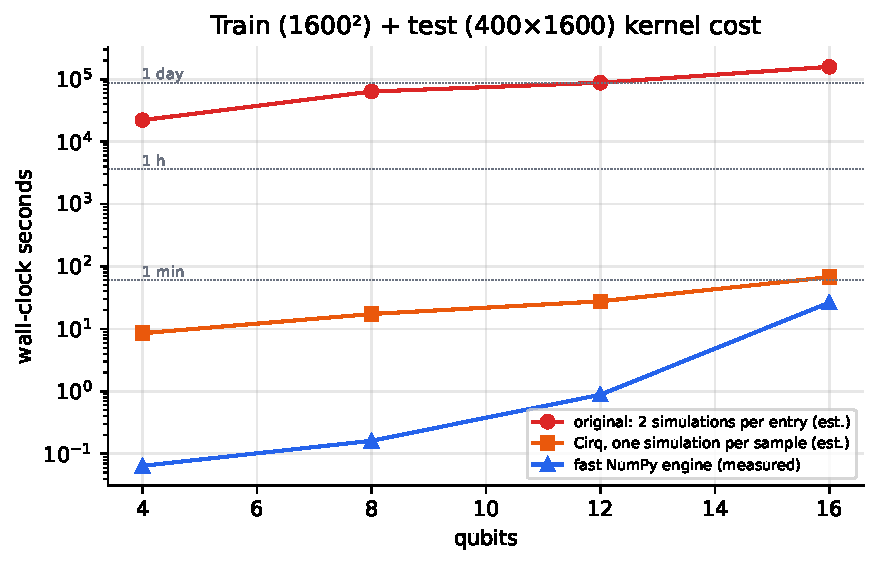
\includegraphics[width=0.72\linewidth]{figures/speed.pdf}
\caption{Wall-clock cost of a full train+test kernel (log scale). Original and Cirq-cached values
are estimates from measured unit costs; fast-engine values are measured end to end.}
\label{fig:speed}
\end{figure}

At 16 qubits the fast engine is limited by memory bandwidth: 2000 states $\times$ 65{,}536
amplitudes $\times$ 8 bytes is about 1\,GB, and the Gram product is about $1.7\times10^{11}$
complex multiply-adds. It is still roughly 6{,}000 times faster than the original, which is what
makes the 5-seed, cross-validated experiments in Section~\ref{sec:results} feasible.
